% ============================================================
%  Sentence Memorability – Report 1
%  Team: Idle Death Gamblers
%  Members: Shreyas Deb, Yajat Lakhanpal, Prasoon Dev
% ============================================================

\documentclass[12pt, a4paper]{article}

% ---- packages -----------------------------------------------
\usepackage[utf8]{inputenc}
\usepackage[T1]{fontenc}
\usepackage{geometry}
\geometry{margin=0.5in}
\usepackage{graphicx}
\usepackage{booktabs}
\usepackage{amsmath}
\usepackage{array}

\usepackage[round]{natbib}
\usepackage[hidelinks]{hyperref}
\usepackage{float}
\usepackage{caption}
\usepackage{subcaption}
\usepackage{parskip}
\usepackage{microtype}
\usepackage{xcolor}
\usepackage[nosep]{enumitem}
\usepackage[compact]{titlesec}
\titleformat{\section}{\large\bfseries}{\thesection}{1em}{}
\titleformat{\subsection}{\normalsize\bfseries}{\thesubsection}{1em}{}
\titleformat{\subsubsection}{\normalsize\itshape}{\thesubsubsection}{1em}{}
\setlength{\textfloatsep}{10pt plus 1.0pt minus 2.0pt}
\setlength{\intextsep}{10pt plus 1.0pt minus 2.0pt}
\setlength{\floatsep}{10pt plus 1.0pt minus 2.0pt}
\linespread{1.1}

\begin{document}

\begin{center}
  \vspace*{-3.5em}
  {\Large \textbf{Report 1: Sentence Memorability Experiment}}\\[6pt]
  {\normalsize \textbf{Idle Death Gamblers}}\\[2pt]
  {\small Shreyas Deb \quad Yajat Lakhanpal \quad Prasoon Dev}
\end{center}
\vspace{0.5em}

% ============================================================
\section{Introduction and Background}
% ============================================================

\subsection{Overview}

Human memory for language is not a faithful archive of words and
syntax. A central finding in cognitive psychology is that listeners
and readers retain the \emph{meaning} of sentences with much greater
fidelity than their verbatim wording or grammatical structure.
This dissociation raises a set of tightly linked empirical questions:
What specific semantic properties of words drive sentence encoding?
Does the grammatical form of a sentence leave an independent trace in
memory? And when surface form is partially forgotten, on what basis do
speakers reconstruct it?

The present study addresses these questions by embedding the three
classic research programmes described below into a single large-scale
online experiment. We examine how the \emph{imageability} (also termed
\emph{memorability} or \emph{imagery value}) of a sentence's constituent
nouns affects (a)~recognition of sentence meaning, and (b)~retention of
grammatical voice, using a continuous recognition paradigm administered
via the internet.

% ------------------------------------------------------------
\subsection{Background and Theoretical Motivation}

Sentence memory can be broadly divided into \textbf{verbatim memory} (the retention of the exact wording and syntactic structure) and \textbf{gist memory} (the retention of the overall meaning). Extensive research demonstrates that gist memory typically lasts much longer than verbatim memory, as people tend to rebuild sentences based on meaning rather than recalling the exact syntactic form.

The earliest and most influential formal account of this phenomenon, the \emph{kernel-plus-tag} hypothesis, was proposed by Miller (1962) and Mehler (1963). This model suggested that sentences are reduced to a stripped-down ``kernel'' proposition, with syntactic features (such as passive voice or negation) stored as independent, forgettable memory trace components. However, \citet{bregman1968} tested and discredited this model. They found that when participants misidentified the syntactic form of a sentence on a first guess, their second guesses still contained information and were reliably above chance ($\chi^2(4) > 20$, $p < .001$). This indicated participants were not retrieving an all-or-none syntactic tag; instead, syntactic form is often reconstructed from other memories, such as imagery and noun salience. 

\citet{begg1971} examined this dissociation directly using a \textbf{continuous recognition paradigm}, which is an approach where participants are presented with a continuous, uninterrupted stream of stimuli. Begg found that the accuracy of meaning judgments decreased with lag ($r = -.996$), while wording judgments were uncorrelated with lag ($r = -.107$). Following Begg and Paivio (1969), who hypothesized that the meaning of a concrete sentence is represented as a spatial image while words are a verbal string, Begg proposed that words are reconstructed from the image at retrieval.

If wording is reconstructed from an image trace, the properties of the words composing that image are critical. \citet{james1973} tested this in a free-recall paradigm using active and passive sentences. They systematically varied the image value of subject and object nouns to create four types of sentences: HH, HL, LH, and LL. They noted a bias where speakers place the most salient aspect of a situation in the subject position, as well as a bias favouring active sentences over passive ones.

Together, this framework suggests that sentence memory is fundamentally semantic and imagistic, wording is reconstructed rather than retrieved, and reconstruction is anchored by the memorability of constituent nouns.

% ------------------------------------------------------------
\subsection{Research Hypotheses}

The present experiment draws upon the continuous recognition paradigm and noun-memorability manipulations to test the following specific hypotheses:

\begin{enumerate}[label=\textbf{H\arabic*:}]
    \item \textbf{(Gist/Meaning):} Sentence memorability (measured via Corrected IR) differs across word memorability conditions (HH, HL, LH, LL).
    \item \textbf{(Verbatim/Wording):} Word recognition accuracy (WR) is independent of the sentence's meaning trace and will not be significantly affected by word memorability conditions.
    \item \textbf{(Voice Effect):} Based on reconstructive biases, active voice sentences will show different memorability/wording recognition patterns compared to passive voice sentences.
\end{enumerate}

% ------------------------------------------------------------
% ------------------------------------------------------------
\subsection{Present Study in Context}

This experiment extends \citet{james1973} from free recall to a continuous recognition paradigm, tests Begg's prediction that memorability selectively affects gist but not wording retention, and does so at large online scale. The dual IR+WR response design allows a within-paradigm dissociation of semantic and syntactic memory traces.

% ============================================================
\section{Methods}
% ============================================================

\subsection{Participants}

Data were collected from online participants via a web-based continuous recognition experiment. A total of 114 participants started the experiment. Two participants failed the validation criterion on all three blocks and were excluded entirely, leaving \textbf{112 participants} in the final sample.

\subsection{Design}

The study used a \textbf{4 (Noun Condition: HH, HL, LH, LL) $\times$ 2 (Voice: Active, Passive)} within-participants design. Noun conditions were defined by crossing the memorability level of the subject and object nouns in each sentence:

\begin{table}[htbp]
  \centering
  \small
  \begin{tabular}{lll}
    \toprule
    \textbf{Code} & \textbf{Subject Noun} & \textbf{Object Noun} \\
    \midrule
    HH & High memorability & High memorability \\
    HL & High memorability & Low memorability \\
    LH & Low memorability & High memorability \\
    LL & Low memorability & Low memorability \\
    \bottomrule
  \end{tabular}
  \caption{The four experimental noun conditions.}
  \label{tab:conditions}
\end{table}

Grammatical voice was fully crossed with noun condition, yielding \textbf{8 within-participant cells}. An additional set of high-frequency filler sentences (coded HF) served as lures for computing false alarm rates.

\subsection{Stimuli}

Simple Subject--Verb--Object (S--V--O) sentences were constructed by systematically varying the memorability of the subject and object nouns. High- and low-memorability nouns were selected from established norms, while verbs were drawn from a fixed set of medium-concreteness action verbs. 

Sentences were kept short (8 words or fewer), contained no proper nouns, and used natural spoken English. They were filtered for semantic coherence and fluency, then manually screened. From the resulting pool, 200 active-voice sentences were selected (50 per condition). Each was converted into a passive-voice form, yielding \textbf{400 target sentences} across 8 conditions. An additional set of HF filler sentences was included to provide false alarm opportunities.

\subsection{Procedure}

Participants completed a \textbf{continuous recognition} task. Each participant saw 48 target sentences across \textbf{3 blocks}. During the task, each sentence was displayed for approximately 4000~ms, followed by an inter-trial interval (gap\_time) of 700--1300~ms. As probes appeared, participants provided judgments regarding whether they recognised the sentence (Immediate Recognition, IR) or whether its grammatical voice matched the original presentation (Wording Recognition, WR).

\subsection{Preprocessing and Data Pipeline}

The raw behavioral data, comprising 81,329 event-log rows, underwent a multi-stage preprocessing pipeline in R to ensure only high-quality, relevant trials were analyzed.

\subsubsection{Data Cleaning and Transformation}

Individual participant log files were combined into a single long-format dataset. The dataset structured the telemetry into explicit columns: \texttt{participant\_ID} (identifier), \texttt{Timestamp} (event time), \texttt{Event} (action type), \texttt{Stimulus} (coded identifier for condition), \texttt{isTarget}, \texttt{isValidation}, \texttt{Accuracy\_IR}, \texttt{Accuracy\_WR}, and reaction times (\texttt{Reaction\_time\_IR}, \texttt{Reaction\_time\_WR}).

We applied the following systematic cleaning steps:
\begin{itemize}[noitemsep]
    \item \textbf{Filtering:} Removed practice-phase trials, inter-stimulus intervals (gap\_time), and rest-phase markers. Outlier removal for reaction times was deliberately not performed to capture the full distribution of natural responses.
    \item \textbf{Trial Scoring:} Calculated binary accuracy for Immediate Recognition (IR) and Wording Recognition (WR) based on button-press values.
    \item \textbf{Feature Extraction:} Stimulus IDs were parsed to extract the factorial levels (HH, HL, LH, LL) and the grammatical voice (Active vs. Passive) of each sentence.
\end{itemize}

\subsubsection{Vigilance Validation}

To ensure participant engagement, each of the three experimental blocks was evaluated using a built-in vigilance formula. Blocks were only retained if they met the following condition:

\begin{equation*}
  \small
  \text{Correct Validations (IRs)} > \left(\frac{\text{Wrong IRs}}{2}\right) + \text{Missed Validations (IRs)}
\end{equation*}

Trials from failed blocks were excluded from the analysis. This process resulted in a final dataset of \textbf{48,281 observations from 112 participants}. The block pass rate was \textbf{96.2\%} (329 out of 342 total blocks), reflecting strong participant adherence to the task instructions.

\subsubsection{Data Quality}

Analysis of the cleaned dataset confirms that the experimental design remained perfectly balanced across the retained trials ($N=112$ participants, 5,264 encoding target trials). Specifically, 110 participants contributed a full complement of 48 target sentences, with only two participants yielding fewer (but still valid) trial counts due to block-level exclusions. Furthermore, stimulus allocation was perfectly factorial: each of the four noun conditions contributed exactly 1,316 encoding trials, and each voice condition contributed exactly 2,632 trials. This resulted in exactly 658 trials per experimental cell ($4 \text{ conditions} \times 2 \text{ voices}$), providing a robust foundation for the within-participants statistical tests.


\subsection{Dependent Variables and Statistical Analysis}

The study evaluated three key metrics:
\begin{enumerate}
    \item \textbf{Corrected IR:} Computed per participant per condition as the Hit Rate minus the global False Alarm Rate. This isolates true recognition discriminability from response bias.
    \item \textbf{WR Accuracy:} For trials with a successful IR press, WR accuracy is the proportion of correct voice judgments.
    \item \textbf{IR Reaction Time:} Extracted in milliseconds from target probe trials.
\end{enumerate}

Normality of the key metrics was assessed using \textbf{Shapiro-Wilk tests}. All metrics showed significant departures from normality ($p < .001$), justifying non-parametric inference throughout.

We conducted Kruskal-Wallis rank-sum tests to assess differences across noun conditions (effect size: $\epsilon^2$), followed by post-hoc Wilcoxon rank-sum tests with Holm correction where applicable. The interaction between noun condition and voice was tested using \textbf{Scheirer-Ray-Hare tests} (the non-parametric analogue of a two-way ANOVA). Voice main effects and chance-level performance were tested using paired and one-sample Wilcoxon signed-rank tests, respectively.

% ============================================================
\section{Results}
% ============================================================

\subsection{Overview}

A total of \textbf{112 participants} contributed data from \textbf{329 validated blocks} (96.2\% pass rate), yielding 896 trial-level observations. The global IR false alarm rate was $M = 0.160$ ($SD = 0.104$, range: $0.00$--$0.43$), reflecting meaningful individual response bias that Corrected IR controls for. All key metrics departed significantly from normality (Shapiro-Wilk: IR~CR $W = 0.941$, $p < .001$; IR~RT $W = 0.986$, $p < .001$; WR~Acc $W = 0.911$, $p < .001$), justifying non-parametric inference throughout.

\subsection{Descriptive Statistics by Condition}

A summary of the descriptive statistics for both metrics across the four noun conditions is provided in Table~\ref{tab:descriptives}.

\begin{table}[htbp]
  \centering
  \small
  \begin{tabular}{lcccc}
    \toprule
    \textbf{Cond} & \textbf{Mean (IR CR)} & \textbf{SD (IR CR)} & \textbf{Mean (WR Acc)} & \textbf{SD (WR Acc)} \\
    \midrule
    HH & 0.689 & 0.210 & 0.747 & 0.208 \\
    HL & 0.691 & 0.200 & 0.747 & 0.209 \\
    LH & 0.679 & 0.209 & 0.762 & 0.203 \\
    LL & 0.632 & 0.224 & 0.730 & 0.220 \\
    \bottomrule
  \end{tabular}
  \caption{Descriptive statistics (Mean and SD) for Corrected IR and WR Accuracy across noun conditions.}
  \label{tab:descriptives}
\end{table}

\subsection{Effect of Noun Condition on Corrected IR}

Per-participant corrected IR scores (hit rate minus false alarm rate, collapsed across voice) by noun condition are visualised in Figure~\ref{fig:ir_cr}.

\begin{figure}[htbp]
  \centering
  
\includegraphics[width=0.85\textwidth]{plots/01_ir_cr_by_condition.png}
  \caption{Corrected Immediate Recognition (IR) scores across the four noun conditions. The LL condition shows a visible deficit compared to the others.}
  \label{fig:ir_cr}
\end{figure}

A Kruskal-Wallis rank-sum test revealed a significant main effect of noun condition on corrected IR, $H(3) = 11.26$, $p = .010$, $\epsilon^2 = 0.013$ (small). Post-hoc Holm-corrected Wilcoxon tests are summarised in Table~\ref{tab:posthoc}. Only the LL condition was significantly lower than HH and HL ($p = .024$ each); the LL--LH gap approached significance ($p = .077$). This threshold pattern indicates a single high-memorability noun is sufficient to anchor sentence gist.

\begin{table}[htbp]
  \centering
  \small
  \begin{tabular}{lccc}
    \toprule
    & \textbf{HH} & \textbf{HL} & \textbf{LH} \\
    \midrule
    HL & 1.000 & & \\
    LH & 1.000 & 1.000 & \\
    LL & .024\textsuperscript{*} & .024\textsuperscript{*} & .077 \\
    \bottomrule
  \end{tabular}
  \caption{Post-hoc pairwise Wilcoxon $p$-values (Holm-corrected). *$p < .05$.}
  \label{tab:posthoc}
\end{table}

\subsection{Effect of Noun Condition on WR Accuracy}

Mean WR accuracy (conditional on a successful IR press) is shown in Figure~\ref{fig:wr_acc}.

\begin{figure}[htbp]
  \centering
  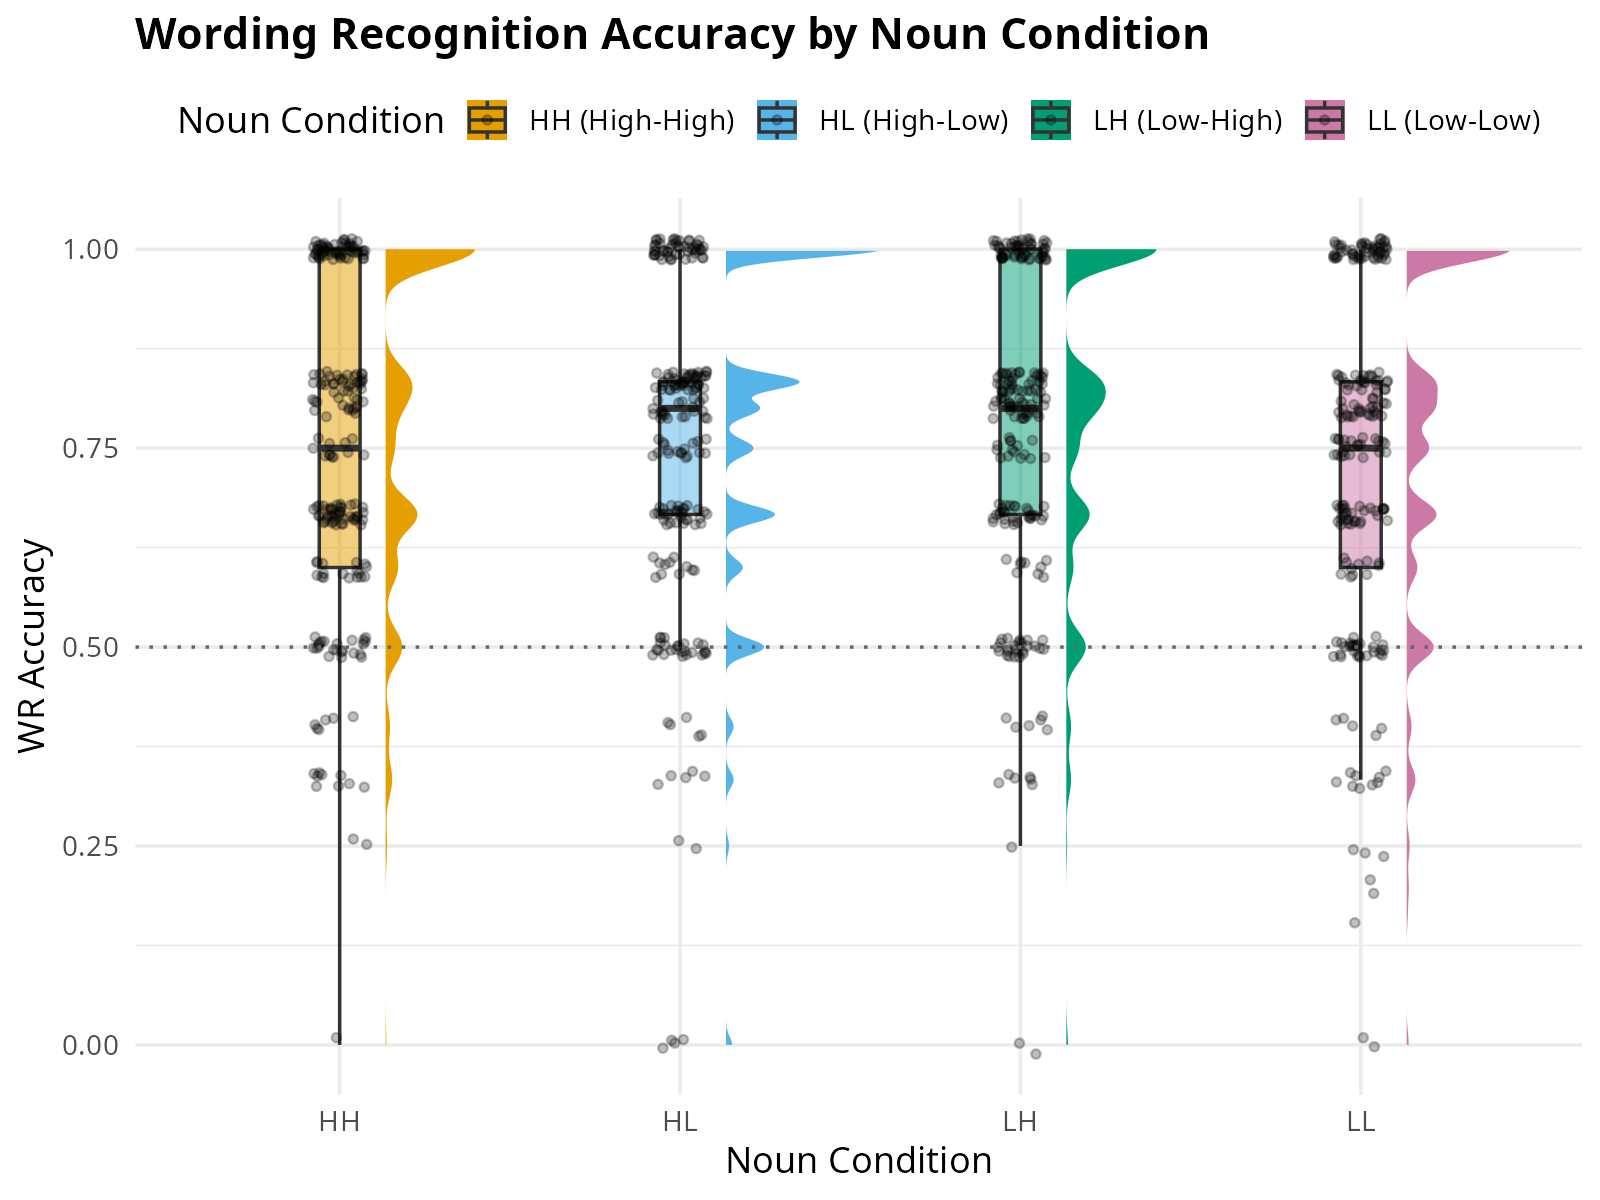
\includegraphics[width=0.85\textwidth]{plots/02_wr_acc_by_condition.png}
  \caption{Wording Recognition (WR) Accuracy across noun conditions. Performance remains high and indistinguishable across all sentence types.}
  \label{fig:wr_acc}
\end{figure}

A Kruskal-Wallis test found \textbf{no significant effect} of noun condition on WR accuracy, $H(3) = 2.52$, $p = .471$, $\epsilon^2 = 0.003$.

\subsection{Noun Condition $\times$ Voice Interaction}

\begin{figure}[htbp]
  \centering
  \begin{subfigure}[b]{0.48\textwidth}
    
\includegraphics[width=\textwidth]{plots/03_ir_cr_condition_x_voice.png}
    \caption{Corrected IR by Condition $\times$ Voice}
  \end{subfigure}
  \hfill
  \begin{subfigure}[b]{0.48\textwidth}
    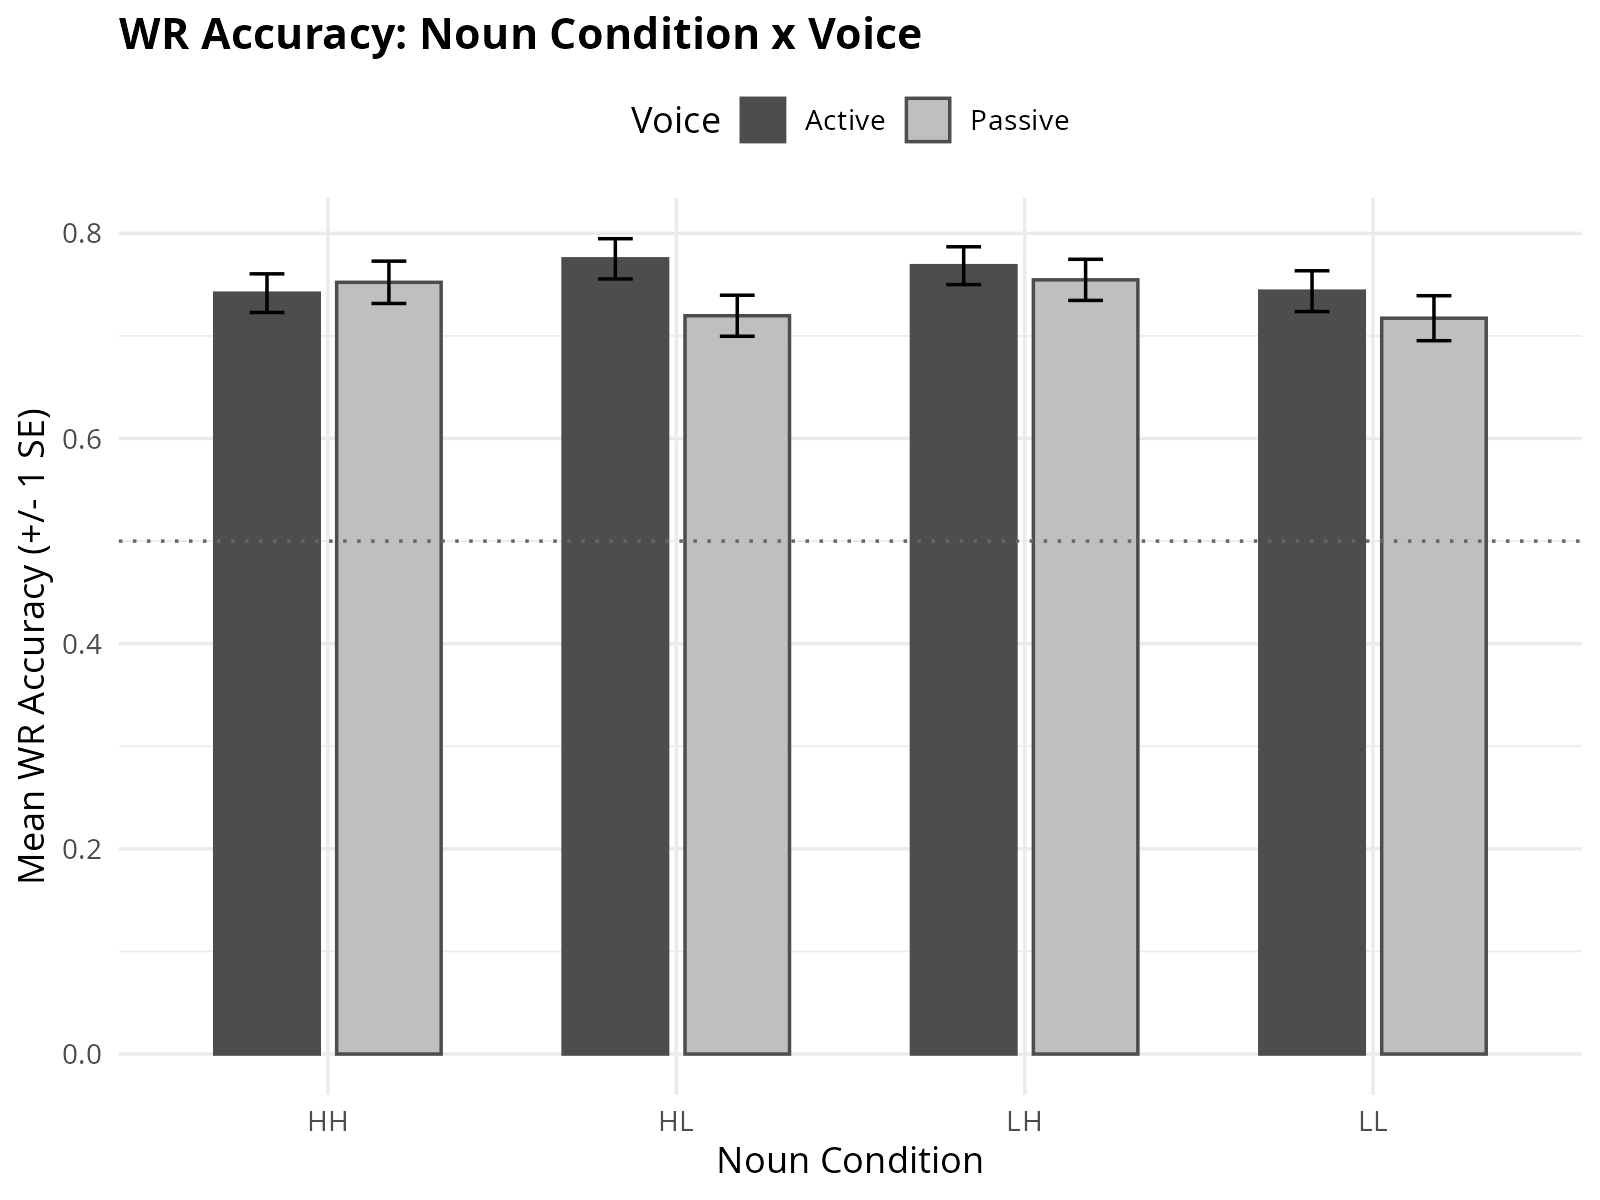
\includegraphics[width=\textwidth]{plots/04_wr_acc_condition_x_voice.png}
    \caption{WR Accuracy by Condition $\times$ Voice}
  \end{subfigure}
  \caption{Interaction plots evaluating whether grammatical voice moderates the memorability effect across tasks.}
  \label{fig:interactions}
\end{figure}

Scheirer-Ray-Hare tests evaluated the noun condition $\times$ voice interaction (Figure~\ref{fig:interactions}). For \textbf{Corrected IR}, we found a main effect of noun condition ($H = 11.26$, $p = .010$), but \textbf{no main effect of voice} ($H = 0.76$, $p = .384$) and \textbf{no interaction} ($H = 0.22$, $p = .975$). For \textbf{WR Accuracy}, there were no significant main effects or interactions (all $p > .200$).

\subsection{Overall Voice Effects and Wording Discriminability}

Paired Wilcoxon signed-rank tests (collapsed across noun conditions) showed no significant voice effect on Corrected IR ($V = 1916.5$, $p = .485$; Active $M = 0.668$, Passive $M = 0.677$) or WR Accuracy ($V = 3520.5$, $p = .114$; Active $M = 0.756$, Passive $M = 0.734$). Notably, the WR direction (active slightly higher) is consistent with the active-sentence recall bias documented by \citet{james1973}, though it does not reach significance here. Figure~\ref{fig:voice_main} shows within-participant differences (Active $-$ Passive), revealing that these distributions are tightly centred on zero.

\begin{figure}[htbp]
  \centering
  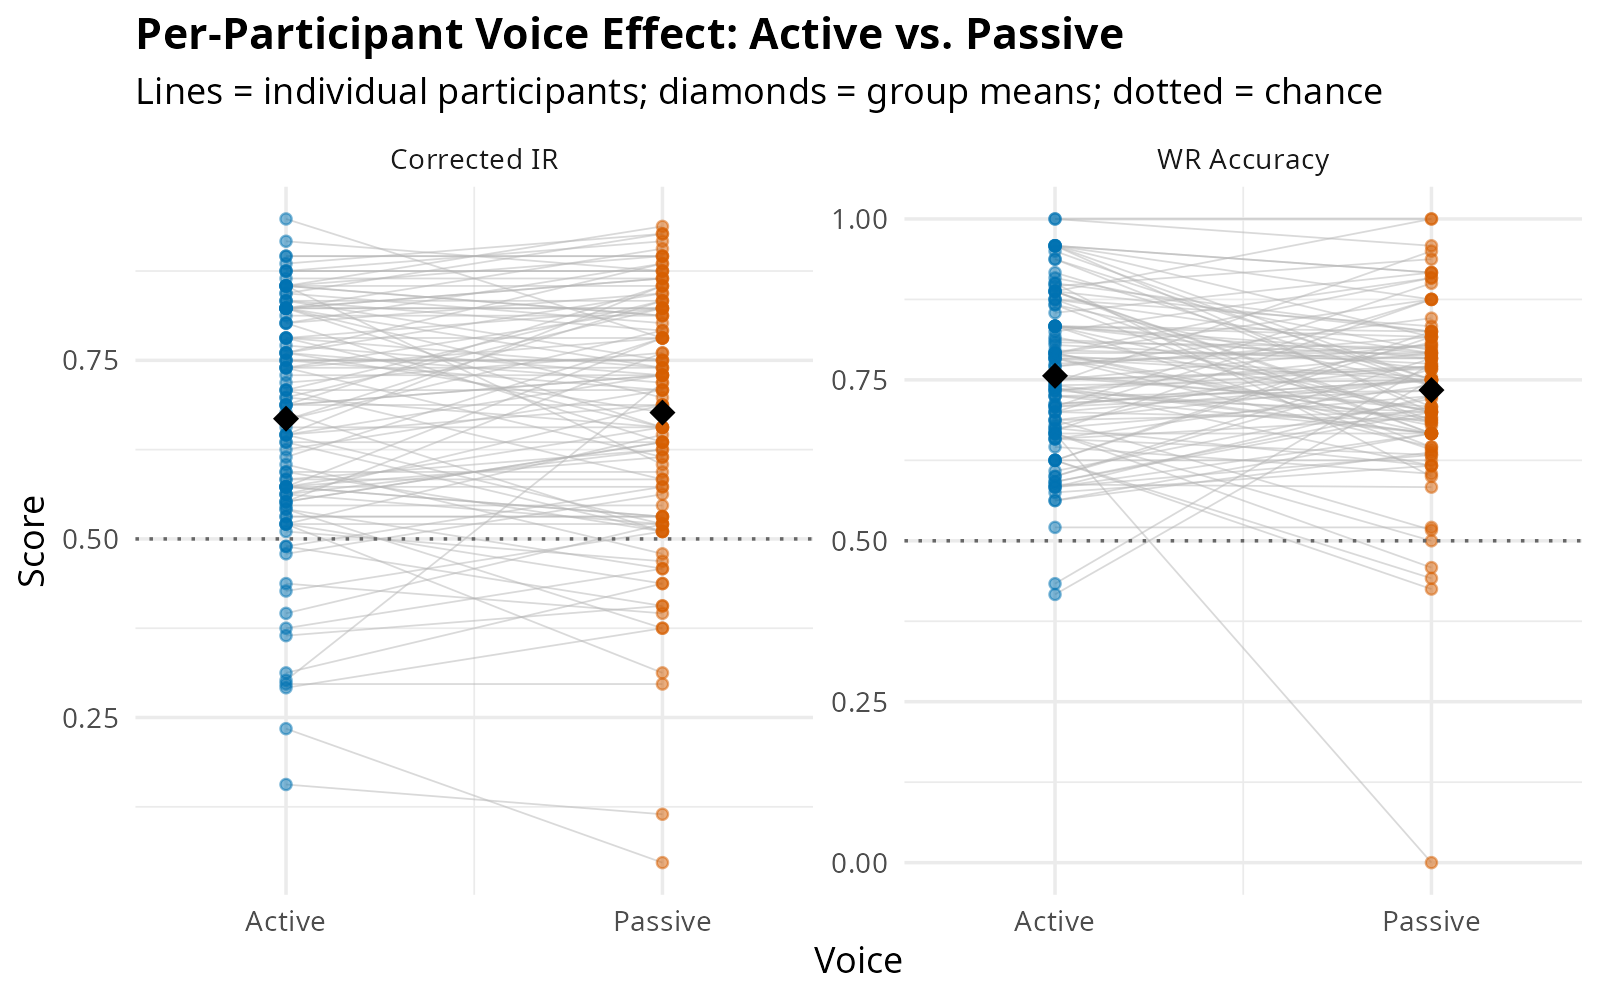
\includegraphics[width=0.9\textwidth]{plots/10_voice_paired_dots.png}
  \caption{Within-participant voice differences (Active $-$ Passive) for Corrected IR (left) and WR Accuracy (right). Both distributions are centred near zero with no systematic skew, confirming no individual-level voice bias. Dashed line = zero effect.}
  \label{fig:voice_main}
\end{figure}

One-sample Wilcoxon tests confirmed WR accuracy significantly exceeded chance~(0.5) for both Active ($V = 6317.5$, $p < .001$) and Passive ($V = 6202$, $p < .001$) voice presentations.

\subsection{Reaction Time and Normality Checks}

\begin{figure}[htbp]
  \centering
  \begin{subfigure}[b]{0.51\textwidth}
    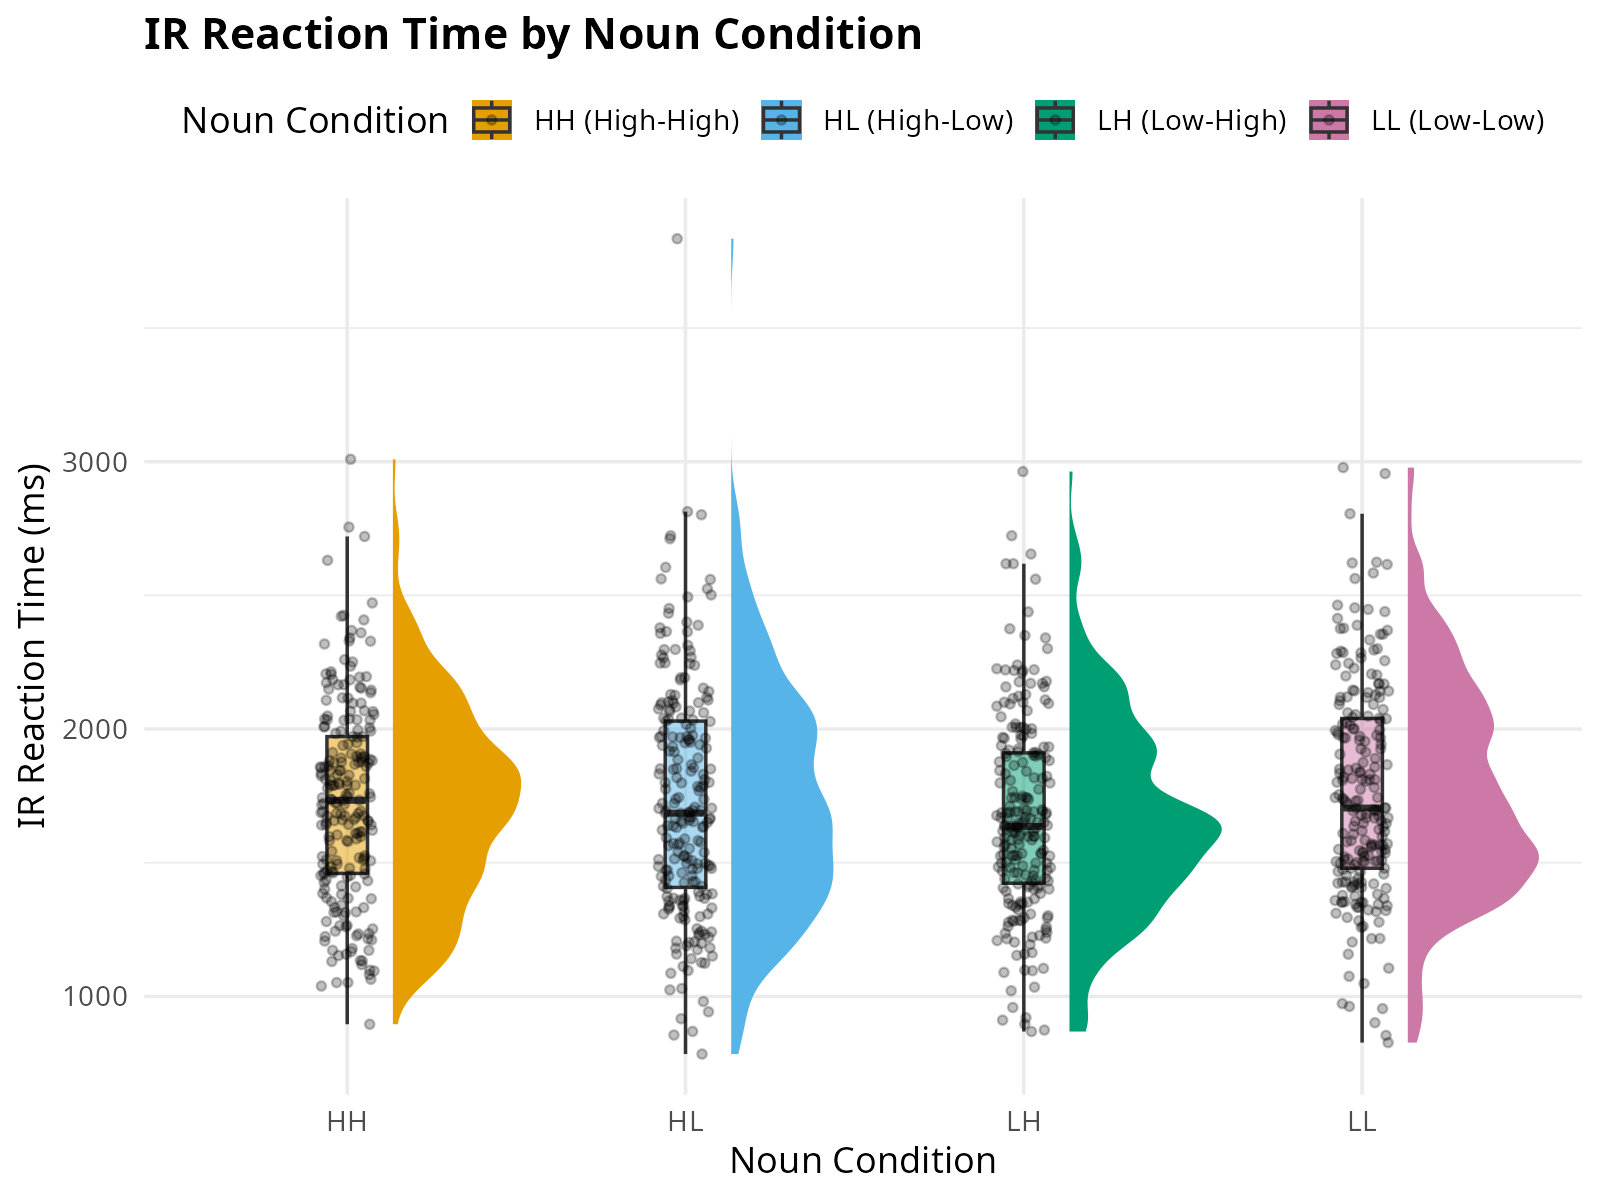
\includegraphics[width=\textwidth]{plots/05_ir_rt_by_condition.png}
    \caption{Reaction Time by Condition}
  \end{subfigure}
  \hfill
  \begin{subfigure}[b]{0.45\textwidth}
    
\includegraphics[width=\textwidth]{plots/06_qq_ir_cr.png}
    \caption{Q-Q Plot for IR CR}
  \end{subfigure}
  \caption{Supplementary reaction time analysis (a) and normality validation (b) supporting the use of non-parametric tests.}
  \label{fig:rt_qq}
\end{figure}

A Kruskal-Wallis test on IR reaction times (Figure~\ref{fig:rt_qq}a) found no significant differences across noun conditions ($H(3) = 6.05$, $p = .109$, $\epsilon^2 = 0.007$). However, the pattern is directionally notable: Passive LL sentences produced the longest mean RT ($M = 1808$~ms) while Active HL sentences were the fastest ($M = 1664$~ms), a 144~ms spread consistent with the hierarchy seen in Corrected IR scores. This trend may become significant with greater power. Q-Q plots (Figure~\ref{fig:rt_qq}b) confirm the heavy-tailed, bounded distributions that necessitated non-parametric tests throughout.

% ============================================================
\section{Discussion and Conclusion}
% ============================================================

This study embedded classic sentence memory paradigms into a large-scale, online continuous recognition task, testing how noun memorability influences both semantic recognition (Corrected IR) and syntactic retention (WR Accuracy).

\subsection{Summary of Findings}

The results support a \textbf{threshold model} of semantic imageability. Corrected recognition was significantly impaired only when \emph{both} the subject and object nouns were of low memorability (the LL condition). The presence of even a single highly memorable noun (HH, HL, or LH) produced uniformly high recognition performance, suggesting that a single vivid anchor is sufficient to reconstruct a sentence's gist. 

Crucially, while noun memorability affected the retention of meaning, it had \textbf{no effect} on wording recognition. WR accuracy was uniformly high and significantly above chance across all conditions. Furthermore, there was no main effect of grammatical voice on either metric, nor was there any interaction between noun memorability and voice. 

\subsection{Theoretical Implications}

These findings align strongly with the dual-process framework proposed by \citet{begg1971}. The dissociation, where noun memorability drives semantic recognition but leaves wording recognition unaffected, supports the notion that meaning is stored holistically (likely as an image trace) while surface wording is reconstructed separately.

Moreover, the lack of an effect for grammatical voice (active vs. passive) during both IR and WR provides further evidence against the kernel-plus-tag hypothesis \citep{bregman1968}. If voice were stored as an independent, fragile tag appended to a core meaning kernel, recognition of passive sentences would likely decay differently or interact with noun saliency. Instead, participants' robust above-chance ability to detect voice mismatches across all conditions suggests that syntactic form is reconstructed at retrieval, anchored by the semantic substance of the remembered event.

\subsection{Future Directions}

Future research should focus on practical, data-driven analyses using the current log files to extract further insights. Specific follow-up steps could include:

\begin{itemize}
    \item \textbf{Multivariate Modeling:} Using Generalized Linear Models (GLMs) to evaluate how multiple predictors (word condition, voice, reaction time, and trial position) jointly influence recognition accuracy.
    \item \textbf{Signal Detection Theory (SDT):} Applying SDT to provide a deeper analysis of sensitivity ($d'$) and response bias ($c$), isolating true discriminability from strategic shifting.
    \item \textbf{Practice Effects:} Comparing participant performance during the practice phase versus the main experimental blocks to evaluate practice and familiarity effects.
\end{itemize}

% ============================================================
%  Code and Data Availability
% ============================================================
\section{Code and Data Availability}

{\small
All raw and processed data, R scripts detailing the data cleaning and statistical analysis pipeline, and source code for this report are available on GitHub: 

\begin{quote}
\url{https://github.com/shrey715/sentence-memorability}
\end{quote}

It is currently private, and thus please reach out to the team for access.

\subsection*{Team Contributions}
\begin{itemize}[noitemsep]
  \item \textbf{Shreyas Deb:} Developed the end-to-end data processing pipeline in R, wrote the scripts for automated data cleaning, validation, and exclusion, and generated all summary visualizations and figures used throughout the report. Shreyas also structured and compiled the final LaTeX document.
  \item \textbf{Yajat Lakhanpal:} Designed and executed the inferential statistical analysis framework, formulating the Kruskal-Wallis omnibus tests, performing all Holm-corrected post-hoc Wilcoxon comparisons, and interpreting the paired voice effect outcomes to support the theoretical claims.
  \item \textbf{Prasoon Dev:} Spearheaded the literature review and theoretical framing, synthesizing foundational work by Bregman \& Stewart (1968), Begg (1971), and James (1973) to formally define the core research hypotheses and map the findings back to reconstructive memory models.
\end{itemize}
}

{\small
\bibliographystyle{plainnat}
\bibliography{references}
}

\end{document}